% !TEX root = supp.tex
% Supplementary material body. Input by supp.tex (standalone PDF; the main PDF no longer carries it).
\renewcommand{\thefigure}{S\arabic{figure}}
\renewcommand{\thetable}{S\arabic{table}}
\paragraph{Reproducibility.}
Every number in the paper maps to a CSV and a configuration file in the released log; the benchmark is 700 lines of Python with no training, and all its model runs fit on one 16 GB GPU in about eight hours. The support head trains in about 25 minutes on one GPU from the released configuration; its runs are logged under the P3 run ids.

\begin{figure}[h]
\centering
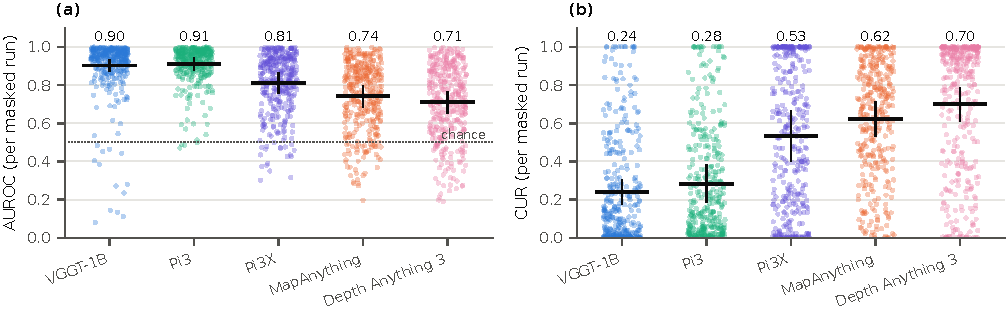
\includegraphics[width=0.95\textwidth]{fig3_metrics}
\caption{\textbf{Per-run spread on DTU.} \auroc{} and \cur{} for every (scan, seed, radius) run under blur and noise fills, with pooled means and intervals. The spread across scans is wide for every model; the intervals in the main tables come from resampling scans.}
\label{fig:metrics}
\end{figure}
\begin{figure}[h]
\centering
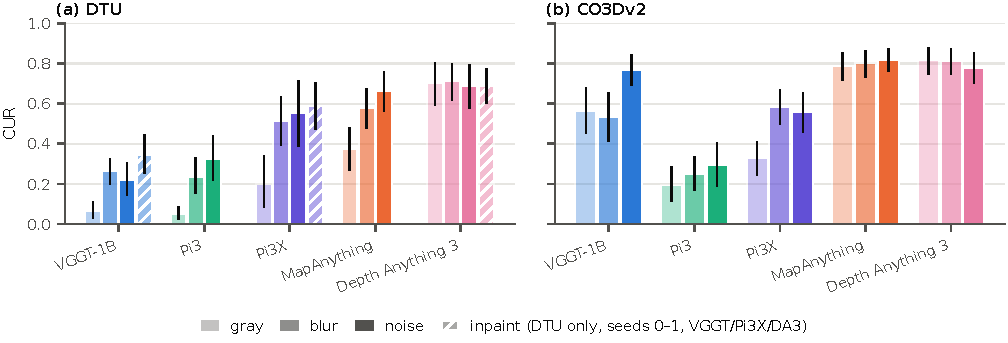
\includegraphics[width=0.95\textwidth]{fig5_fills}
\caption{\textbf{Fill ablation.} \cur{} per model and fill on DTU and CO3Dv2 (five seeds) and for the inpainted fill on DTU (two seeds, three models). A visible gray patch gives the lowest leakage; natural-statistics and inpainted fills give more.}
\label{fig:fills}
\end{figure}
\begin{figure}[h]
\centering
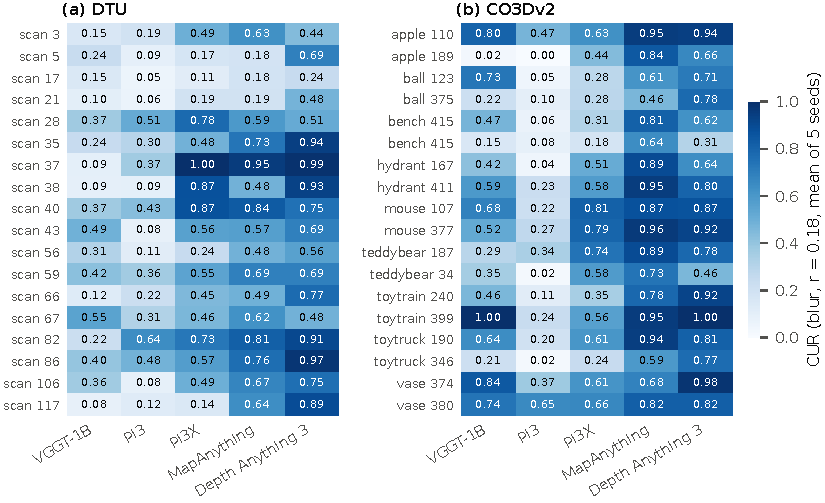
\includegraphics[width=0.95\textwidth]{fig7_perscene}
\caption{\textbf{Per-scene \cur{}} (blur fill, radius 0.18, mean over seeds) for every model on DTU scans and CO3Dv2 scenes. Rows are scenes, columns are models.}
\label{fig:perscene}
\end{figure}

\paragraph{Pre-registered gates.}
The pass conditions were written into the run registry before the corresponding heads were trained, and the registry is versioned with the code. Gate 3 (true-visibility head; written 2026-11-06, before any visibility head was trained; the training kernels ran from commit \texttt{4132d11}): the head counts as detecting missing support when, pooled over 3, 5 and 10 views on DTU, (a) it beats native confidence on \auroc{} and \cur{} (paired sign-flip $p<0.05$), (b) it beats its per-image control on \auroc{} by at least 0.02 at $p<0.05$, and (c) both conditions hold on at least one dataset the head never saw (CO3Dv2 or ETH3D); if (b) fails, the single-view-support signal is reported as recoverable from per-image features and the method claim is dropped. Gate 4 (label-free head; written 2026-11-06 16:51 UTC, before any label-free head was trained, commit \texttt{c7e6919}): on DTU and on CO3Dv2, (a) and (b) as above against its own per-image control, and (c) within 0.03 \auroc{} of the ground-truth-trained head on DTU and ahead of reprojection consistency on CO3Dv2 at $p<0.05$ (its training signal is the reprojection test, so it has to generalise better than its teacher); if (a) or (b) fails the head is dropped, if only (c) fails it is reported as an ablation. The earlier Gate 2 (fill-trained head) had the clause ``head ahead of the control at $p<0.05$'' with no margin; it passed by the letter on differences of 0.0004 and 0.003 and the paper does not count it, which is why Gate 3 carries a margin.

\paragraph{Gaussian-splatting backbone (partial run).}
AnySplat~\cite{anysplat}, a feed-forward 3D Gaussian-splatting model, was scored on the DTU configuration with its per-pixel Gaussian opacity as confidence (120 of 540 rows) and with the rendered accumulated alpha (450 of 540 rows), bf16 on one L4, run P3-gs. Pooled over blur and noise: opacity \auroc{} 0.583 / \cur{} 0.718, rendered alpha 0.632 / 0.745, \curerr{} 0.02 and 0.06; the noise fill drives the opacity below chance (0.36). The representation does not change the answer: a Gaussian the model places on an unseen surface is as opaque as one on an observed surface. The run stopped behind other jobs on the shared card and is reported as partial.

\paragraph{Run registry.} Every table cell maps to a run id (P1-full, P2-full, P2-stress, P2-co3d, P2-co3d-b, P3-pv-smoke, P2-smoke-b, P3-native, P3-reproj, P3-pv, P3-oia-dtu, P3-oia-abl, P3-oia-stress-*, P3-kaggle-vggt) whose CSV, configuration JSON and kernel log are released with the code, together with the dated log of every failed run and every correction.
